% The IA error budget of Roman cosmic shear: how wrong may the FLAMINGO
% intrinsic-alignment spectra be, scale by scale, before Omega_m or S8 moves
% by 0.3 sigma; and how NLA and TATT compare with it.
% Build with the summary-notes skill: assets/build_note.sh notes/ia_error_budget
\documentclass[11pt]{article}

\usepackage[margin=1in]{geometry}
\usepackage{amsmath}
\usepackage{amssymb}
\usepackage{graphicx}
\usepackage{booktabs}
\usepackage{xcolor}
\usepackage[font=small,labelfont=bf,labelsep=period]{caption}
\usepackage[hidelinks]{hyperref}

% Let figures share pages with text instead of leaving float-only pages.
\renewcommand{\topfraction}{0.9}
\renewcommand{\bottomfraction}{0.7}
\renewcommand{\textfraction}{0.1}
\renewcommand{\floatpagefraction}{0.8}

% Symbols, one macro per object.
\newcommand{\hMpc}{\,h\,{\rm Mpc}^{-1}}
\newcommand{\kuv}{k_{\rm UV}}
\newcommand{\PNL}{P_{\rm NL}}
\newcommand{\PdE}{P_{\delta E}}
\newcommand{\PEE}{P_{EE}}
\newcommand{\Om}{\Omega_{\rm m}}
\newcommand{\T}{^{\mathsf{T}}}
\newcommand{\bvec}[1]{\boldsymbol{#1}}

% =====================================================================
% Numbers
% =====================================================================
% Part 1: results (analysis/roman_dchi2/v8/: clean_budget.json,
% nonlinear_tol.json, fid_fits.json; 13 November 2026), production truth
% unless stated. Part 2: inputs.
%
% Statements that rest on Part 1; re-check after a rerun:
%   - without a cut the budget is a few to 15% for one k range and about
%     2% for a coherent error, at every k up to about 3 h/Mpc (Summary;
%     "The budget");
%   - with the cut it is 6 to 18% (GI) at k <= 0.2 and opens above k_UV;
%   - without a cut both models leave the budget from k ~ 0.1 to 0.2,
%     with the cut both stay inside ("The models against the budget").
\newif\ifnumbersfinal
\numbersfinaltrue
\newcommand{\refresh}[1]{\ifnumbersfinal#1\else\textcolor{red}{#1}\fi}
% ---------------------------------------------------------------------
% Part 1: results.
\newcommand{\SigOmNone}{\refresh{0.0036}}
\newcommand{\SigSNone}{\refresh{0.0020}}
\newcommand{\SigOmCut}{\refresh{0.0080}}
\newcommand{\SigSCut}{\refresh{0.0068}}
% budget, no cut (percent): one k range, GI and II; coherent steps
\newcommand{\BumpNoCutLo}{\refresh{3}}
\newcommand{\BumpNoCutHi}{\refresh{15}}
\newcommand{\AboveNoCutGI}{\refresh{1.5 to 2}}
\newcommand{\BelowNoCutGI}{\refresh{2 to 3}}
% budget, K_0 = 0.3 (percent)
\newcommand{\BumpCutGILo}{\refresh{6}}
\newcommand{\BumpCutGIHi}{\refresh{18}}
\newcommand{\BumpCutIILo}{\refresh{7}}
\newcommand{\BelowCutGI}{\refresh{9}}
\newcommand{\BelowCutII}{\refresh{18}}
% verification: full refits at linear tolerances (sigma)
\newcommand{\VerLo}{\refresh{0.27}}
\newcommand{\VerHi}{\refresh{0.33}}
% the models (fitted at the fiducial cosmology), production truth, percent
\newcommand{\NLANoCutGILow}{\refresh{+10}}
\newcommand{\NLANoCutIILow}{\refresh{+16}}
\newcommand{\TATTNoCutGILow}{\refresh{+4}}
\newcommand{\TATTNoCutIILow}{\refresh{+10}}
\newcommand{\NLANoCutGIMid}{\refresh{+22}}
\newcommand{\NLANoCutIIMid}{\refresh{-9}}
\newcommand{\TATTNoCutIIMid}{\refresh{-5}}
\newcommand{\CutGILow}{\refresh{-2}}
\newcommand{\CutIILow}{\refresh{-7}}
\newcommand{\NLACutIIMid}{\refresh{-28}}
\newcommand{\TATTCutIIMid}{\refresh{-15}}
% Roman fits with the cut, cosmology free (sigma): production and stitched
\newcommand{\ProdNLAS}{\refresh{+0.24}}
\newcommand{\ProdTATTS}{\refresh{+0.24}}
\newcommand{\StNLAOm}{\refresh{-0.29}}
\newcommand{\StTATTOm}{\refresh{-0.22}}
% ---------------------------------------------------------------------
% Part 2: inputs.
\newcommand{\Tol}{0.3}

\begin{document}

\begin{center}
  {\LARGE The IA error budget of Roman cosmic shear\par}
  \vspace{0.6em}
  {\large How wrong may the FLAMINGO alignment spectra be before
    $\Om$ or $S_8$ moves by \Tol$\sigma$?\par}
  \vspace{0.6em}
  {\large November 2026\par}
  \ifnumbersfinal\else
    \vspace{0.6em}
    {\color{red}Numbers in red are being refreshed.\par}
  \fi
\end{center}
\vspace{1em}

\section{Summary}
\label{sec:summary}

\paragraph{The question.}
The FLAMINGO GI and II power spectra are injected into the Roman cosmic-shear
data vector. If they are wrong by a fraction $\varepsilon$ in some range of
$k$, how large may $\varepsilon$ be before the best-fit $\Om$ or $S_8$ moves
by more than \Tol{} of its marginalized error? And where do NLA and TATT sit
against that budget?

\paragraph{The budget.}
Without a scale cut, one range of $k$ may be wrong by \BumpNoCutLo{} to
\BumpNoCutHi\%, and a coherent error over all smaller (or all larger) scales
by only about 2\%, at every $k$ up to about $3\hMpc$; beyond that the 2.5
arcmin angular limit of the data hides the spectra. With the production cut
$\kuv = 0.3/D(z)$, one range at $k \le 0.2\hMpc$ may be wrong by \BumpCutGILo{}
to \BumpCutGIHi\% (GI), a coherent error over every kept scale by about
\BelowCutGI\% (GI) and \BelowCutII\% (II), and errors above $k \simeq 0.3$ to
$1\hMpc$ are not seen at all (Figure~\ref{fig:bands}).

\paragraph{The models.}
Fitted to FLAMINGO at the fiducial cosmology, both NLA and TATT leave the
budget from $k \simeq 0.1$ to $0.2\hMpc$ without a cut; TATT is the closer
of the two at $k \simeq 0.1$ to 0.5. With the cut, both stay inside it at
every $k$ (Figure~\ref{fig:overlay}), and their fitted shifts are below
\Tol$\sigma$ (production truth: $S_8$ moves by \ProdNLAS$\sigma$ for both).
With the cut the two models are nearly indistinguishable, because the kept
scales are the ones both describe equally well.

\section{Setup}
\label{sec:setup}

\paragraph{Truths.}
Two versions of the FLAMINGO IA spectra, at the FLAMINGO D3A cosmology
($\Om = 0.306$, $10^9 A_s = 2.099$, $n_s = 0.967$, $H_0 = 68.1$, $\Omega_b =
0.0486$):
\begin{itemize}
  \item \textbf{production}: a smoothing spline of the measured $\PdE$ and
    $\PEE$ at every $k \ge 0.05\hMpc$ (held below);
  \item \textbf{stitched}: NLA below a transition scale $k_t(z)$ (0.16 to
    $0.27\hMpc$ over $0.2 \le z \le 2$) and the same spline above,
    $R_X = (1 - w) R_X^{\rm NLA} + w R_X^{\rm FL}$, with $R_X = P_X/\PNL$ and
    $w$ a logistic step in $\ln k$ at $k_t$.
\end{itemize}
Both are injected into cosmolike as tables (the sim-IA path), so the truth
and every model share the Limber integrals and the Hankel transforms.

\paragraph{Data.}
Roman $\xi_\pm$, 8 tomographic bins and 15 angular bins from 2.5 to 250
arcmin, 1080 points, with the production covariance \texttt{example1\_cov}.
Two cuts: none, and the production IR/UV mask $\kuv = 0.3/D(z)$ (an angular
bin is kept when less than 5\% of its signal comes from $k > \kuv$).

\paragraph{The analysis model is the truth itself.}
To make the budget independent of any IA model, the model fitted to the
perturbed data is the truth, with only an overall IA amplitude and a
power-law redshift evolution free, besides the cosmology:
\begin{equation}
  \PdE \to a(z)\,\PdE^{\rm truth},\qquad
  \PEE \to a(z)^2\,\PEE^{\rm truth},\qquad
  a(z) = A\left(\frac{1+z}{1.62}\right)^{\eta},
  \label{eq:model}
\end{equation}
with $\Om$, $A_s$, $A$, $\eta$ free. At $A = 1$, $\eta = 0$ it reproduces the
data exactly, so every shift below is caused by the perturbation alone.

\paragraph{The criterion.}
A perturbation is within budget when $|\delta\Om|/\sigma(\Om) < \Tol$ and
$|\delta S_8|/\sigma(S_8) < \Tol$, with $\sigma$ the marginalized errors:
$\sigma(\Om) = \SigOmNone$ and $\sigma(S_8) = \SigSNone$ without a cut,
\SigOmCut{} and \SigSCut{} with it.

\section{The perturbations}
\label{sec:pert}

A perturbation multiplies one spectrum (GI or II) by $1 + \varepsilon f(k)$,
the same at every redshift, with $f \ge 0$, so the spectrum moves in one
direction only ($\varepsilon > 0$ too high, $\varepsilon < 0$ too low).
Three shapes, each centered on a scale $k_c$ from 0.01 to $10\hMpc$:
\begin{align}
  \text{one $k$ range wrong:}\quad & f = \exp\!\left[-\frac{\ln^2(k/k_c)}{2\cdot0.3^2}\right],\\
  \text{every scale larger than $k_c$ wrong:}\quad & f = \left[1 + e^{\ln(k/k_c)/0.25}\right]^{-1},\\
  \text{every scale smaller than $k_c$ wrong:}\quad & f = \left[1 + e^{-\ln(k/k_c)/0.25}\right]^{-1}.
\end{align}
The first is a bump about a factor of 1.4 wide; the other two are smooth
steps.

\paragraph{How the tolerance is found.}
$\xi_{\rm IA}$ is linear in the injected tables, so the change of the data
vector, $\delta\bvec d = \varepsilon\,\bvec r_f$, is computed exactly: each
$f$ is written on 61 narrow tents in $\ln k$, each tent's response is one
cosmolike run, and the responses add. The fit responds as
\begin{equation}
  \delta\bvec p = \varepsilon\, F^{-1} J\T C^{-1} \bvec r_f,
  \qquad F = J\T C^{-1} J + \Pi^{-1},
  \label{eq:resp}
\end{equation}
with $J$ the Jacobian of the model~\eqref{eq:model} in $(\Om, A_s, A, \eta)$
and $\Pi$ Gaussian priors on $A$ and $\eta$ of the chain-prior width. The
tolerance is the $\varepsilon$ at which $\delta\Om$ or $\delta S_8$ reaches
\Tol$\sigma$. Full non-linear refits at the tolerances land at \VerLo{} to
\VerHi$\sigma$ up to $\varepsilon \simeq 20\%$. Above 20\% (only at $k \lesssim
0.6\hMpc$ with the cut, mostly II) the refit moves far and the linear values,
also after a refit-based search, overestimate the limit; those points are
upper estimates.

\section{The budget}
\label{sec:budget}

Figure~\ref{fig:bands} shows the budget for the production truth; the
stitched truth gives the same figure to within 10\%, because the budget is
set by the size of the IA signal and the precision of the data, which the two
truths share.

\begin{figure}[tbp]
  \centering
  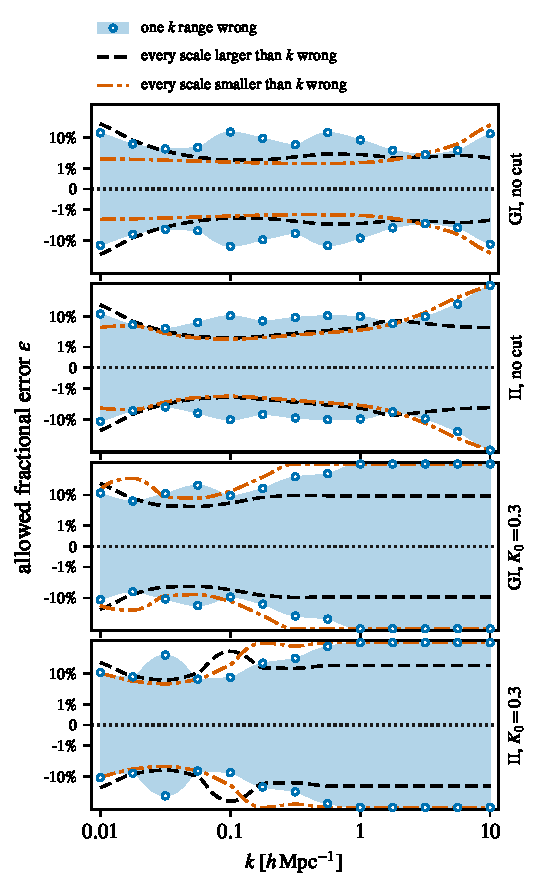
\includegraphics[width=3.5in]{plots/bands_prod/bands_prod.pdf}
  \caption{The error budget of the production FLAMINGO IA spectra: the
    fractional error, positive (too high) or negative (too low) and the same
    at every redshift, that keeps $\Om$ and $S_8$ within \Tol$\sigma$.
    Shaded with markers: one $k$ range wrong; black dashed: every scale
    larger than $k$ wrong; vermillion dash-dot: every scale smaller than
    $k$ wrong. Panels: GI and II, without a cut and with $\kuv = 0.3/D(z)$.
    Symmetric logarithmic axis (linear within $\pm1\%$; the panel edges are
    $\pm100\%$, no limit).}
  \label{fig:bands}
\end{figure}

\paragraph{Without a cut: about 1 to 15\% everywhere.}
One $k$ range may be wrong by \BumpNoCutLo{} to \BumpNoCutHi\%, a coherent
error over every smaller scale by \AboveNoCutGI\% (GI), over every larger
scale by \BelowNoCutGI\%, at every $k$ up to about $3\hMpc$. Two facts set
this level. In FLAMINGO the alignment is strong (amplitude $A_1 \simeq 3.4$),
so IA is 20 to 55\% of $\xi_\pm$; and with every point kept Roman measures
$S_8$ to 0.25\%. A 1\% IA error is then a 0.3\% change of the data, which
moves $S_8$ by a sizable fraction of its error unless the free amplitude
absorbs it, and an error confined to some range of $k$ is not an amplitude
change. Above $3$ to $5\hMpc$ the budget opens because the data stop at 2.5
arcmin, which those wavenumbers project below.

\paragraph{With the cut: room above $\kuv$, and about 10\% below.}
The cut removes the small-angle bins, so errors at $k \gtrsim 0.3$ to
$1\hMpc$ no longer matter (100\% in Figure~\ref{fig:bands}). The kept scales,
which feed the large-angle bins, still constrain the IA: one range at $k \le
0.2\hMpc$ may be wrong by \BumpCutGILo{} to \BumpCutGIHi\% in GI and from
\BumpCutIILo\% in II, and a coherent error over every kept scale by about
\BelowCutGI\% in GI and \BelowCutII\% in II. Large scales are not more
fragile than small ones; they are simply the scales every cut keeps.

\section{The models against the budget}
\label{sec:models}

NLA ($A_1$, $\eta_1$) and TATT ($A_1$, $\eta_1$, $A_2$, $\eta_2$, $b_{\rm TA}$),
with power-law redshift evolution, are fitted to the FLAMINGO data vector at
the fiducial cosmology (IA parameters only), with the same cut as the
panel. Their error against the truth,
\begin{equation}
  \Delta_X(k, z) = \frac{P_X^{\rm model}(k, z)}{P_X^{\rm truth}(k, z)} - 1,
\end{equation}
is drawn over the budget in Figure~\ref{fig:overlay} (production truth) and
Figure~\ref{fig:overlays1} (stitched truth), averaged over the core
redshifts $0.2 \le z \le 2$ with its range.

\begin{figure}[tbp]
  \centering
  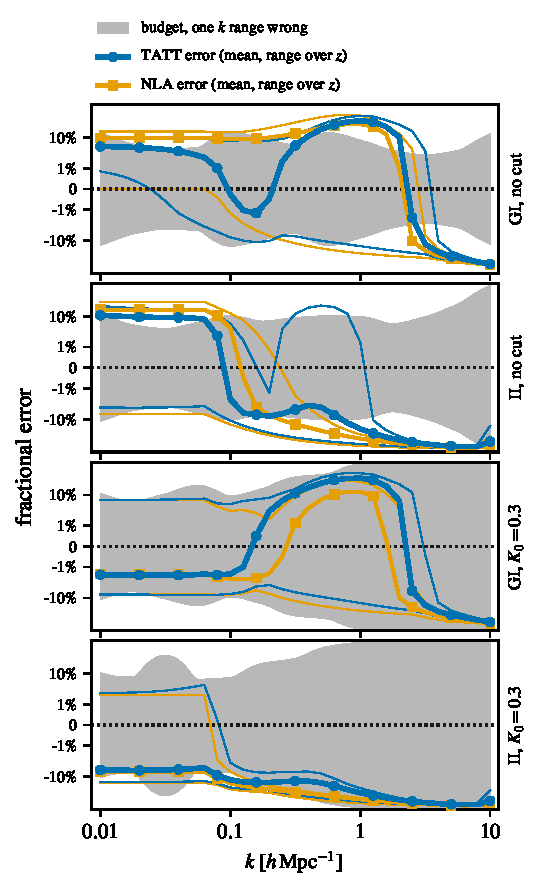
\includegraphics[width=3.5in]{plots/overlay_prod/overlay_prod.pdf}
  \caption{NLA (orange, squares) and TATT (blue, circles) against the
    production FLAMINGO truth, over the budget for one $k$ range wrong
    (gray). Thick: the error averaged over the core redshifts; thin: its
    smallest and largest value over them. Each model is fitted at the
    fiducial cosmology with the cut of its panel.}
  \label{fig:overlay}
\end{figure}

\paragraph{Without a cut both models fail beyond $k \simeq 0.1$ to 0.2.}
NLA is \NLANoCutGILow\% too high in GI and \NLANoCutIILow\% in II at $k \le
0.06\hMpc$, at or beyond the edge of the budget, \NLANoCutGIMid\% in GI at 0.3
to $1.5\hMpc$ and 50 to 90\% too low beyond $2\hMpc$. TATT is closer at
large and intermediate scales (\TATTNoCutGILow\% in GI and \TATTNoCutIILow\%
in II at $k \le 0.06$, within $\pm3\%$ in GI at 0.1 to 0.2, and
\TATTNoCutIIMid\% against \NLANoCutIIMid\% in II at 0.1 to 0.6), but fails
the same way above $0.3\hMpc$. Without a cut neither model is usable; the
difference between them sits at $k \simeq 0.1$ to 0.5.

\paragraph{With the cut both stay inside.}
Both are \CutGILow\% off in GI and \CutIILow\% in II at $k \le 0.06\hMpc$,
inside a budget of about 10\%, and \NLACutIIMid\% (NLA) and \TATTCutIIMid\%
(TATT) in II at 0.1 to 0.6, where the budget is wider. Above $0.3\hMpc$ they
are 10 to 90\% off, where the cut has removed the data. Their fitted shifts
with the cut, cosmology free, agree: on the production truth $S_8$ moves by
\ProdNLAS$\sigma$ for NLA and \ProdTATTS$\sigma$ for TATT, on the stitched
truth $\Om$ moves by \StNLAOm{} and \StTATTOm$\sigma$. The band bounds one
range of $k$ wrong at a time, while a model is wrong at every $k$ at once;
its fitted shift is the final test, and it is just under \Tol.

\begin{figure}[tbp]
  \centering
  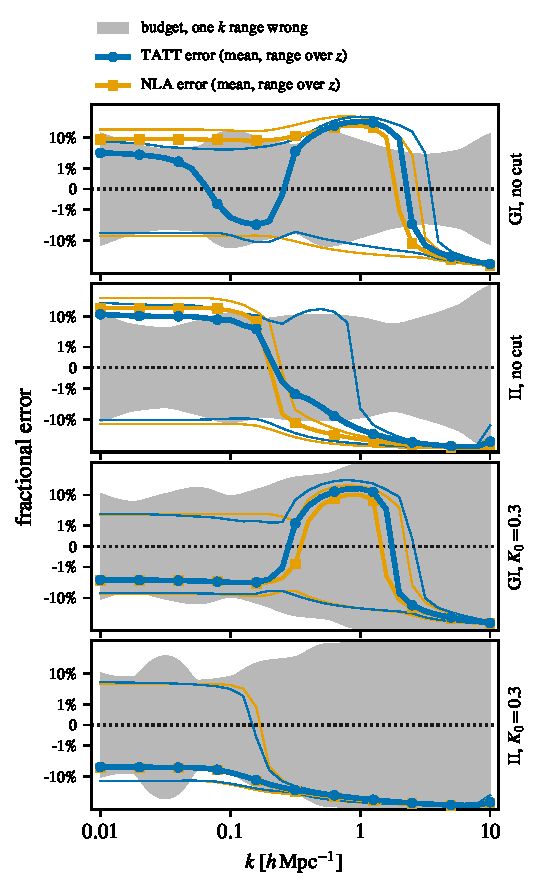
\includegraphics[width=3.5in]{plots/overlay_s1/overlay_s1.pdf}
  \caption{As Figure~\ref{fig:overlay}, for the stitched truth (NLA below
    the transition scale $k_t(z)$). With the cut, the large-scale error of
    either model is only the mismatch between its power-law redshift
    evolution and the amplitude of each snapshot.}
  \label{fig:overlays1}
\end{figure}

\appendix

\section{Numerical checks}
\label{app:checks}

\begin{itemize}\sloppy
  \item \textbf{Build.} cocoa-cosmolike-core and cocoa\_roman\_real (cocoa
    v5.x) with the sim-IA patches of \texttt{cosmolike\_patches/}, compiled
    with \texttt{-DSIM\_KMIN\_HMPC=1e-6 -DSIM\_KMAX\_HMPC=0}; the injected
    $\xi_{\rm IA}$ agrees with the earlier build to $10^{-3}$.
  \item \textbf{Responses.} The 61 tent responses sum to $\xi_{\rm IA}$ to
    $4\times10^{-10}$; the analytic form of the model~\eqref{eq:model},
    $\sum_s a_s \bvec r_{{\rm GI},s} + a_s^2 \bvec r_{{\rm II},s}$, matches
    cosmolike to $10^{-9}$.
  \item \textbf{Linear response.} Full Gauss--Newton refits (cosmology
    through CAMB at every step) at 16 tolerances below 20\% give \VerLo{} to
    \VerHi$\sigma$ in the limiting parameter.
  \item \textbf{A cosmolike pitfall.} Once sim-IA tables are loaded, a
    native call with every IA amplitude at zero still returns the injected
    IA; the pure GG vector is computed before any table is loaded.
  \item \textbf{Fits without a cut} with the cosmology free move it by 10
    to 30$\sigma$, where its linearized response in the fitter fails; the
    model errors therefore use fits at the fiducial cosmology, where TATT
    fits better than NLA as a nested model must ($\chi^2 = 1169$ against
    1462 for 1080 points).
\end{itemize}

\section{Where the code and results are}
\label{app:code}

Paths relative to \texttt{analysis/roman\_dchi2/v8/} of the repository.

\begin{center}
  \small
  \begin{tabular}{ll}
    \toprule
    step & script $\rightarrow$ output \\
    \midrule
    linear budget, checks, Roman fits & \texttt{clean\_budget.py} $\rightarrow$ \texttt{clean\_budget.json} \\
    tolerances above 10\% by refitting & \texttt{nonlinear\_tol.py} $\rightarrow$ \texttt{nonlinear\_tol.json} \\
    NLA and TATT at the fiducial cosmology & \texttt{fid\_fits.py} $\rightarrow$ \texttt{fid\_fits.json} \\
    figure data & \texttt{notes/ia\_error\_budget/plots/make\_figure\_data.py} \\
    \bottomrule
  \end{tabular}
\end{center}

\section{Open issues}
\label{app:open}

\begin{itemize}
  \item Tolerances between about 20 and 100\% at $k \lesssim 0.6\hMpc$ with
    the cut are upper estimates (Section~\ref{sec:pert}).
  \item The perturbations are the same at every redshift; a model's error
    varies with redshift, which the budget does not represent.
  \item One simulation and one galaxy selection, with a strong alignment
    ($A_1 \simeq 3.4$); the fractional budget scales roughly as $1/A_1$ for
    GI and $1/A_1^2$ for II.
\end{itemize}

\end{document}
